\documentclass[11pt,a4paper]{article}
\usepackage[T1]{fontenc}
\usepackage[utf8]{inputenc}
\usepackage{lmodern,microtype,amsmath,amssymb,bm,booktabs,graphicx}
\usepackage[margin=25mm]{geometry}
\usepackage[numbers,sort&compress]{natbib}
\usepackage[colorlinks=true,allcolors=blue]{hyperref}
\hypersetup{pdftitle={MOUSE: Semiempirical Orbital-Optimized DFT with Analytic Gradients and Hessians},pdfauthor={Vincenzo Barone}}
\usepackage{siunitx}
\usepackage{fancyhdr}
\pagestyle{fancy}\fancyhf{}\fancyhead[L]{MOUSE: semiempirical orbital-optimized DFT}\fancyhead[R]{IJQC submission}\fancyfoot[C]{\thepage}
\setlength{\headheight}{14pt}
\renewcommand{\topfraction}{0.90}\renewcommand{\bottomfraction}{0.85}\renewcommand{\textfraction}{0.08}\renewcommand{\floatpagefraction}{0.70}
\newcommand{\npi}{\ensuremath{n\!\rightarrow\!\pi^*}}
\newcommand{\pipi}{\ensuremath{\pi\!\rightarrow\!\pi^*}}
\newcommand{\Eh}{\ensuremath{E_{\mathrm h}}}
\title{Semiempirical Orbital-Optimized DFT in MOUSE:\\Spin-Pure Excited-State Surfaces with Analytic Gradients and Hessians}
\author{Vincenzo Barone\\\small Consorzio Interuniversitario Nazionale per la Scienza e Tecnologia dei Materiali}
\date{5 November 2026}
\begin{document}
\maketitle
\begin{abstract}
Excited-state spectroscopy of large molecules requires a balanced description
of electronic reorganization and nuclear motion. We present a semiempirical
orbital-optimized model in the Molecular Orbital Utility for Semiempirical
Explorations (MOUSE), in which spin-polarized GFN2 (second-generation
geometry, frequency, noncovalent and tight-binding) orbitals are
relaxed on a density functional theory (DFT)-informed energy surface and
singlet excitations are formed
from spin-pure configurations. The excitation energy, forces and vibrational
curvature are obtained from the same state-specific surface. Selected double
excitations and a screened interaction describe the multiconfigurational
character of conjugated chromophores while preserving a compact valence
representation. On 26 states in 24 molecules, the mean absolute error is
0.183 eV with a maximum error of 0.478 eV. The twelve $\pi\!\rightarrow\!\pi^*$
states have a mean absolute error of 0.209 eV, and the fourteen
$n\!\rightarrow\!\pi^*$ states have a mean absolute error of 0.160 eV.
Analytic gradients and Hessians include orbital relaxation, spin recoupling,
configuration-space response, the moving ground-state projector and
state-interaction response. The resulting energy surface supports excited-
state relaxation, vibrational analysis and repeated calculations on extended
chromophores. Carotene and chlorophyllide examples illustrate the treatment of
strongly conjugated pigment manifolds.
\end{abstract}
\noindent\textbf{Keywords:} orbital-optimized DFT; semiempirical quantum
chemistry; excited states; spin-pure ROKS; analytic gradients; analytic
Hessians; DeltaSCF; MOUSE.

\section{Introduction}
The absorption spectrum of a conjugated molecule is determined by the coupled
motion of electrons and nuclei. The transition changes bond orders, charge
distribution and orbital occupations, and the electronic state therefore
relaxes on a geometry different from that of the ground state. Excited-state
structures and vibrational spectra require an energy surface that describes
this relaxation together with its first and second nuclear derivatives. The
same requirement appears in pigment photophysics, where several close-lying
configurations share the visible spectrum and their ordering determines the
observed bands.

A practical description must retain the electronic degrees of freedom of the
chromophore and remain affordable for conformational sampling, solvent
models and multilevel QM/QM$'$ calculations. Semiempirical methods provide
this reach through compact valence Hamiltonians. Their value for excited
states is greatest when the approximation defines a differentiable,
state-specific energy rather than only a vertical transition estimate.
Analytic gradients and Hessians then connect spectroscopy with structures,
relaxation pathways and vibronic observables. Subtractive multilayer
constructions such as ONIOM provide an established framework for combining
quantum levels.\cite{oniom2015}

The field includes simplified response theories such as sTDA, sTDA-xTB and
the recent std2 family, DFTB-based response and $\Delta$DFTB, TDDFT+TB,
TDDFT-aas, and semiempirical multireference methods based on OMx/ODMx.
\cite{tda,stdft2014,stdaxtb2016,std22026,dftb2025,deltadftb2016,tbgrad2023,aas2024,omxexc2016,odmx2019}
These methods establish complementary routes to efficient spectra, excited-
state gradients and multiconfigurational wave functions. The present work
focuses on the state-specific energy surface generated by orbital relaxation
and its analytic nuclear response.

Simplified Tamm--Dancoff and TD-DFT methods describe many transitions from a
ground-state reference and are effective for broad spectral surveys.\cite{tda,stdft2014,stdaxtb2016}
State-specific orbital optimization provides a complementary description: a
non-Aufbau occupation defines the excited configuration, the orbitals relax in
its field, and the transition energy is the difference between stationary
ground- and excited-state energies. In $\Delta$SCF and orbital-optimized DFT,
this relaxation is central to charge-transfer, $n\!\rightarrow\!\pi^*$ and
strongly reorganized $\pi\!\rightarrow\!\pi^*$ states.\cite{mom2008,hait2021}
The excited solution is an electronic stationary point and often a saddle;
direct orbital optimization and saddle searches therefore provide a natural
route to state following.\cite{levifaraday,levi2020,ivanov2021,gmf2023}

State-specific optimization is already possible at the semiempirical level. In particular, $\Delta$DFTB provides self-consistently optimized excited-state energies and gradients, with applications to structures, Stokes shifts and vibrational frequencies.\cite{deltadftb2016} The opportunity addressed here is therefore more specific than introducing semiempirical $\Delta$SCF. We seek a DFT-informed semiempirical OO-DFT surface with explicit spin polarization, a spin-pure singlet representation, and complete analytic response through the nuclear Hessian. For a single targeted state, such a formulation allows the existing ground-state engine to supply most of the electronic machinery, while the excited-state solver supplies occupation control, orbital stationarity and its constrained response. For interacting or strongly mixed configurations, an additional state-interaction treatment is required.

Our organizing principle is to separate the standard ground-state DFT calculation from the less expensive calculation of the excitation response or energy increment. Writing $\Delta E_I=E_I-E_0$ distinguishes the description of the absolute ground-state energy from the description of the change produced by excitation. In a multilevel application, this separation can be expressed schematically as $E_I^{\rm composite}=E_0^{\rm DFT}+\Delta E_I^{\rm low}$: standard DFT supplies the baseline, while a compact quantum model supplies the state-dependent increment. This expression is a design principle for combining levels of theory, rather than an assumption that the two terms have the same approximation error. It also requires consistent differentiation of both contributions when forces or frequencies of the composite surface are needed.

In the present MOUSE formulation, a conventional DFT program prepares ground-state orbital-reference information and response operators at an anchor geometry. These quantities are transferred to a native GFN2-based valence representation and then used by a separate prepared excited-state calculation.\cite{gfn2} The native spatial orbitals remain the variational variables. Ground and excited states are made stationary in a common prepared semiempirical energy, and their difference defines the reported excitation increment. This provides a concrete separation between external reference preparation and runtime evaluation: the latter uses the semiempirical engine and stored operators, without a new DFT or TDA calculation. Reuse of the prepared operators away from the anchor is an approximation whose range must be validated. The multilevel motivation likewise does not imply that an additional DFT ground-state calculation is included in every benchmark timing.

MOUSE implements this strategy with a spin-polarized native energy and a
restricted-open-shell Kohn--Sham (ROKS) singlet construction.\cite{roks1998}
A coherent combination of exchanged-spin determinants defines a spin-pure
configuration state function (CSF); its orbitals satisfy the constrained
excited-state stationarity equations. Selected singlet double excitations are
coupled through a prepared screened interaction to describe configuration
mixing beyond a single optimized promotion. The resulting surface requires
the response of the stationary orbitals, constraint multipliers, nonorthogonal
configuration metric, ground-state projector and state-interaction
eigenvector. These contributions give analytic gradients and Hessians of the
energy used for the spectrum.

This work establishes the semiempirical OO-DFT formulation and its analytic
implementation in MOUSE. TDA is evaluated on the same corrected native GFN2
orbitals and reference preparation, allowing the role of orbital relaxation
and state interaction to be measured directly. The study covers vertical
excitation energies, state following, analytic derivatives and conjugated
pigment manifolds. Figure~\ref{fig:workflow} summarizes the relation between
the molecular excitation, the state-specific energy surface and its nuclear
response.

\begin{figure}[!htbp]
\centering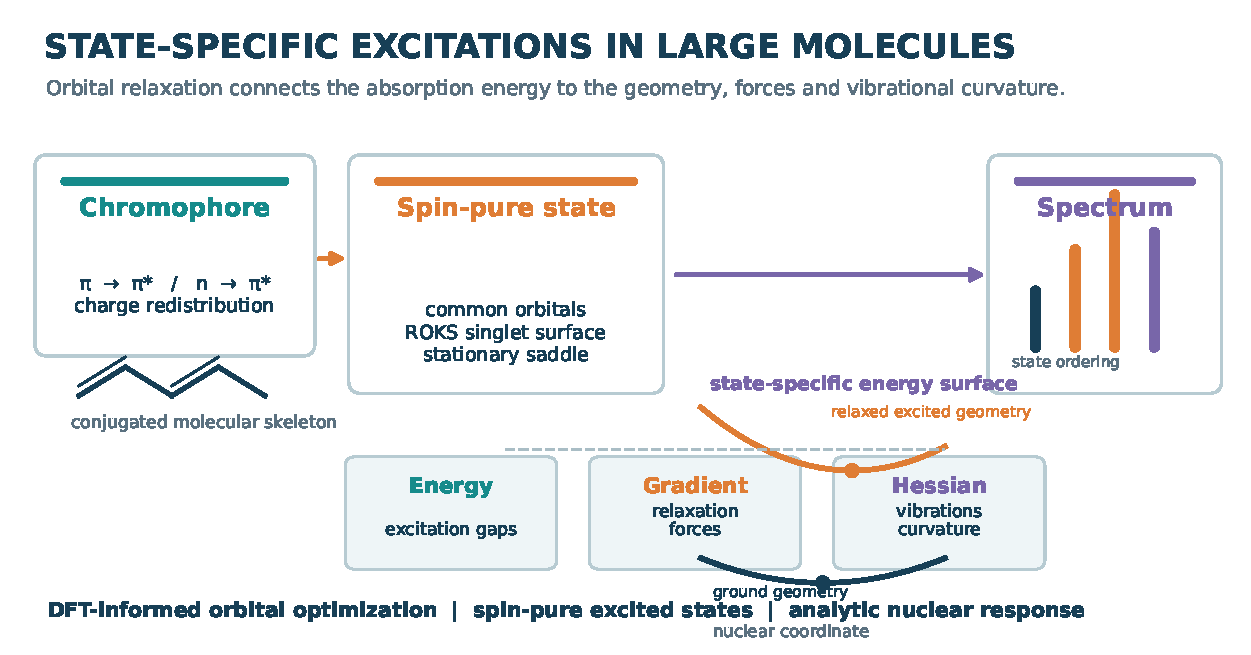
\includegraphics[width=\linewidth]{figures/graphical_abstract_ijqc.pdf}
\caption{Chemical and spectroscopic picture of the MOUSE excited-state surface. Orbital relaxation converts a vertical excitation into a state-specific energy surface that supplies the absorption energy, relaxed forces and vibrational curvature. Spin-pure singlet configurations and their interaction describe the ordering and intensity pattern of conjugated chromophores.}\label{fig:workflow}
\end{figure}

\section{Theory and implementation}
\subsection{Common reference and spin-polarized native energy}
The native GFN2 spatial orbitals $C_{\rm n}$ define the retained valence
orbital space. At the frozen anchor, a core-orthogonal isometry embeds this
space in the
DFT AO space. The diagonal Rayleigh quotients of the embedded DFT Fock matrix
supply levels $F_i$. Qualified occupied/virtual assignments transfer DFT
orbital spacings to $Q_i$ after aligning occupied centroids; levels without a
levels retain $F_i$. The correspondence thresholds are 0.7 in absolute
overlap and 0.05 in best-versus-alternative margin. If the molecular Q
transfer loses its occupied--virtual gap, Q reverts to F. The common
one-body reference uses $\epsilon_i=(F_i+Q_i)/2$ before orbital optimization.
DFT spatial orbitals are not substituted for the native orbitals. This is
not an arithmetic average of two independently optimized excited energies.

In a complete symmetric AO-pair moment representation, the prepared energy is
\begin{align}
 E[P^\alpha,P^\beta;R]&=E_{\rm native}
 +v^{\mathsf T}q+\tfrac12(q-q_0)^{\mathsf T}K_c(q-q_0)
 +\tfrac12m^{\mathsf T}K_s m,\\
 q_a&=\operatorname{Tr}[B_a(P^\alpha+P^\beta)],\qquad
 m_a=\operatorname{Tr}[B_a(P^\alpha-P^\beta)].
\end{align}
$E_{\rm native}$ retains the native electronic, charge-dependent,
anisotropic, repulsive, dispersion and spin-polarization terms; $K_c$ and
$K_s$ are the prepared additional response corrections. The charge correction
subtracts the corresponding native response rather than adding a duplicate
Coulomb kernel. The linear term places the reference Fock spectrum in the
native orbital space. The quadratic tensors are prepared at the stationary embedded
DFT density and the linear reference is centered on the native ground.
Spin polarization is part of the energy and its derivatives, not an additive
excitation correction.

The final reference is CAM-B3LYP,\cite{camb3lyp2004} with range parameter
$0.33\,{\rm bohr}^{-1}$. The inherited uracil scale $\lambda=0.9$ multiplies
its exact-exchange response once, giving short- and long-range response
coefficients 0.171 and 0.585. The semilocal response is unchanged and orbital
gaps are not multiplied by $\lambda$. Neither operator construction nor
state assignment uses a reference excitation energy.

\subsection{Spin purity and electronic saddle stationarity}
For a promotion $h\to p$, the two exchanged-spin determinants sharing a
single spatial orbital set define a singlet CSF with a consistent fermion
phase convention. Its energy is the restricted-open-shell multiplet sum
\begin{equation}
 E_S(C,R)=2E_M(C,R)-E_T(C,R).
\end{equation}
The singlet CSF is spin pure, whereas the density-functional multiplet-sum
energy remains approximate. This does not identify a broken-symmetry
$M_s=0$ determinant as an exact singlet. Four-open-shell occupations require
two independent singlet recouplings, both retained below.

The ground is made stationary in the native closed-shell functional. Target
ROKS orbitals satisfy the ground-CSF orthogonality constraint and their
bordered stationarity equations. Metric-preserving orbital rotations,
Newton residual searches, and state-overlap guards locate the assigned
branch. An excited solution may be an electronic saddle, as emphasized in
the direct-optimization work of Levi and co-workers;\cite{levi2020,gmf2023}
no orbital-energy minimum is assumed. Electronic saddle order and nuclear
vibrational stability are distinct properties.

Figure~\ref{fig:saddle} illustrates the distinction between electronic
stationarity and nuclear relaxation.

\begin{figure}[tbp]\centering
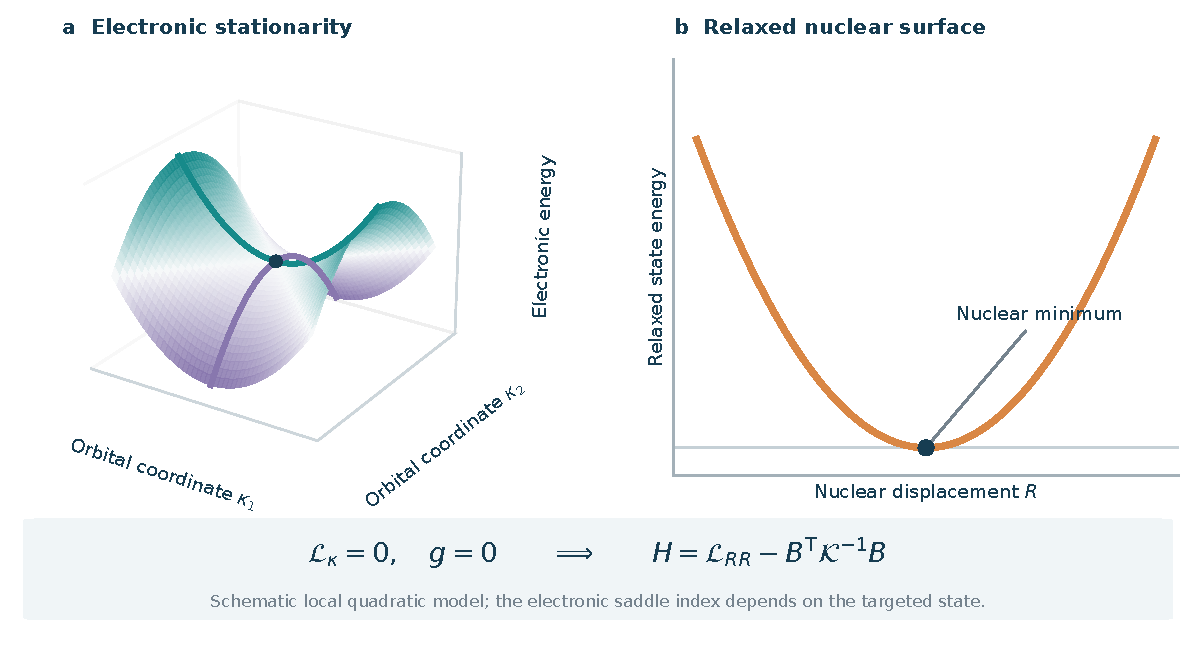
\includegraphics[width=\linewidth]{figures/stationary_response.pdf}
\caption{Electronic saddle character and relaxed nuclear curvature are
distinct properties of an excited-state surface.}\label{fig:saddle}
\end{figure}

\subsection{Analytic response of the state-interaction surface}
Let $z$ collect the stationary ground and target orbital coordinates and
constraint multipliers, and write their residual equations as
$F(z(R),R)=0$. Their first and second analytic responses obey
\begin{align}
 F_z z_a&=-F_a,\\
 F_z z_{ab}&=-F_{ab}-F_{az}z_b-F_{bz}z_a-F_{zz}[z_a,z_b].
\end{align}
The bordered linear systems are solved on the regular assigned branch.
Both responses are required: the subsequent state-interaction eigenvalue
is not stationary with respect to the individually optimized ROKS orbitals.
A variational single-determinant Hessian formula alone would omit terms.

For the generalized eigenproblem in the moving ground-orthogonal space,
$Hc=\mathcal E Sc$ with $c^{\mathsf T}Sc=1$, total matrix derivatives give
\begin{align}
 \mathcal E_a&=c^{\mathsf T}(H_a-\mathcal E S_a)c,\\
 \mathcal E_{ab}&=c^{\mathsf T}(H_{ab}-\mathcal E S_{ab})c
 -\mathcal E_b c^{\mathsf T}S_a c-\mathcal E_a c^{\mathsf T}S_b c\nonumber\\
 &\quad+2\sum_{k\ne n}
 \frac{[c_k^{\mathsf T}(H_a-\mathcal E S_a)c]
 [c_k^{\mathsf T}(H_b-\mathcal E S_b)c]}{\mathcal E-\mathcal E_k}.
\end{align}
Here the derivatives include the orbital/multiplier responses, metric,
transported operators, and moving ground projector. The relevant metric
and eigenvalue separations must be resolved. The absolute excited-state
energy defines molecular forces and curvature; vertical excitation energies
subtract the stationary native ground. Finite differences enter only the
independent validation of these analytic derivatives.

\section{Computational protocol}
The assessment contains 26 valence transitions in 24 molecules. Reference
energies are the QUEST theoretical best estimates.\cite{quest,quest2025}
Molecular geometries and target identities are fixed throughout the
assessment, which spans carbonyl, heteroaromatic and conjugated chromophores.

The prepared CAM-B3LYP references retain the archived aug-cc-pVDZ AO basis,
numerical grid level 3, frozen core embedding, and native valence space.
DFT transition information supplies assigned-state seeds and character checks.
Completed references, stationary states and operators are reused.

The calculations were performed on verified remote compute hosts. Runtime
property checks use two BLAS threads per process. The parallel nuclear-column
validation limits concurrent processes and preserves every completed column.

Matched TDA controls use the same stationary native GFN2 spatial orbitals,
F/Q one-body preparation, density-response kernel and $\lambda=0.9$:
\begin{equation}
 A_{ia,jb}=(\epsilon_a-\epsilon_i)\delta_{ij}\delta_{ab}+K_{ia,jb}.
\end{equation}
The complete nonlocal singlet $A$ operator is used, including the exchange
contribution missing from a real symmetrized static response. These controls
are distinct from published sTDA-xTB and from a separately optimized TDA
parameterization. The screened interaction introduced below is an additional
ingredient of OO-CID, not a hidden modification of the reported TDA values.

\section{Selected optimized-target and double-excitation model}
The final development step replaces the auxiliary canonical-singles manifold
by a compact selected OO-CID space: the requested optimized, ground-orthogonal
ROKS singlets, their paired doubles, canonical frontier double excitations,
and the two exact four-spin singlets. Unoptimized auxiliary canonical singles
are omitted by excitation rank, using the same rule for every molecule.
This model-space choice was selected using thirteen exposed states. It is
an empirical design choice, not a proof that auxiliary singles always worsen
an orbital-optimized calculation. The common one-body reference averages
Fock Rayleigh quotients and qualified DFT orbital levels \emph{before} orbital
optimization, with weights $1/2,1/2$. This differs from averaging two separately
optimized parent energies. The exchange-response scale remains $\lambda=0.9$.
There is no orbital-gap scaling or fitted excitation offset.

Let $S_{IJ}$ be the CSF metric, $H^0_{IJ}$ the physical Slater--Condon
matrix element, and $d_I=E_I-H^0_{II}/S_{II}$. Away from the exact four-spin
block defined above, the effective matrix is
\begin{equation}
 H_{IJ}=H^0_{IJ}+\tfrac12 S_{IJ}(d_I+d_J).
\end{equation}
The native density functional supplies $E_I$ including spin polarization.
The excited-sector basis is projected orthogonal to the moving stationary
ground CSF $|0\rangle$, using
$|\widetilde I\rangle=|I\rangle-|0\rangle S_{0I}/S_{00}$.
We solve the resulting generalized eigenproblem and subtract the independently
stationary native ground energy. We differentiate this projector as well as
the CSF metric; using an unprojected full-SI root and shifting its energy is
not equivalent. The off-diagonal construction remains an approximate
state-interaction functional; it does not supply a universally balanced
multi-determinant ground-state functional.

The selected rule was frozen in commit \texttt{467a9e5} before evaluating
nitrosomethane and maleimide. All fifteen transitions satisfy the unchanged
aggregate MAE gate of 0.3 eV and individual error gate of 0.5 eV, with an MAE
of 0.220 eV and maximum absolute error 0.498 eV. The two post-freeze errors
are $-0.002$ and $+0.402$ eV, respectively, giving 0.202 eV MAE. These
molecules appeared in older campaigns: this is prospective validation of
the frozen candidate on historically exposed molecules, not a blind study.
Glyoxal is within only 0.002 eV of the individual gate; passing that gate
must not be interpreted as a universal correction to all $n\pi^*$ errors.
The same-reference, same-native-orbital TDA control gives 0.966 eV MAE over
these fifteen states. This control isolates the present kernel and is not
a claim to outperform every calibrated TDA or sTDA parameterization.

\begin{figure}[tbp]\centering
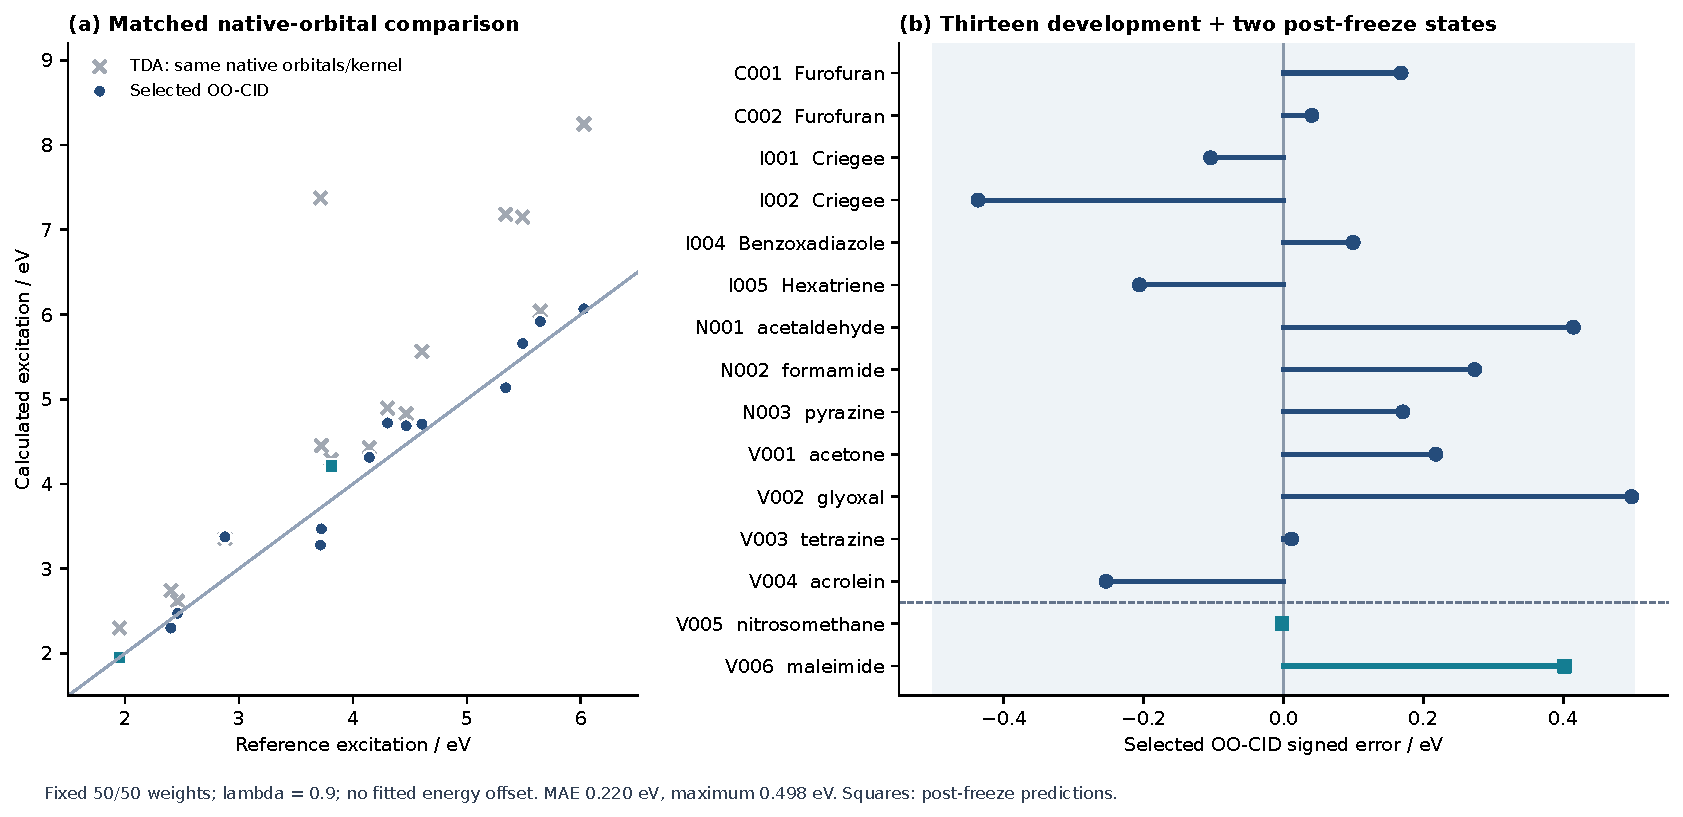
\includegraphics[width=\linewidth]{figures/selected_cid_validation.pdf}
\caption{Final selected OO-CID predictions. The shaded error interval is
$\pm0.5$ eV. Thirteen states informed model selection; squares identify the
two predictions made after the final candidate freeze. All controls use
native GFN2 spatial orbitals.}\end{figure}

The public class \texttt{PreparedNOSIModel} evaluates a portable, checksummed
MOUSE surface. LINK selects it with \texttt{nosi\_50\_50}. It uses native ground-program
Fock, energy and derivative machinery, constrained orbital optimization,
and a small CSF eigenproblem. It performs no TDA solve, DFT-backend import,
or fresh ground-state SCC calculation during evaluation. One-time DFT
reference preparation is still required. APOC follows coherent determinant
sums, preserving their phases and checking $\langle S^2\rangle=0$ using
$\|S_+\Psi\|^2$, rather than assigning spin purity to an $M_s=0$ determinant.
Only accepted LINK geometries advance an atomic, model-identified restart;
trial geometries leave that restart unchanged.

Complete analytic Hessians of the final selected model are verified for
Criegee (two states, 15 coordinates), glyoxal (one state, 18 coordinates),
and furofuran (two states, 36 coordinates). Independent reoptimized energy
checks at two displacement sizes and directions validate the first and
second derivatives; these finite differences are validation only. The largest Richardson-extrapolated
errors are $1.33\times10^{-10}$ Hartree/bohr for directional gradients and
$3.28\times10^{-7}$ Hartree/bohr$^2$ for directional curvatures. Both
first and second implicit KKT responses, the moving ground projector,
metric and generalized eigenvector response are retained. Physical operators
and auxiliary orbitals remain fixed in the co-rotating orthonormal AO frame;
this precisely defines an anchored PES, not a re-canonicalized model.
A fresh-process public-API Hessian reproduces the Criegee research matrices
within $9.1\times10^{-13}$ Hartree/bohr$^2$, taking 40.82 s with two BLAS
threads and 262 MiB peak RSS on MAC-STUDIO. Its energy-only evaluation takes
0.135 s. These timings exclude preparation and do not establish a vertical
speed advantage over TDA. The earlier 42.22 s phthalimide Hessian belongs
to the preceding production model, not this final selected candidate.

This completes a finite candidate test and automatic derivative integration.
It does not demonstrate an independent broad CT/Rydberg benchmark, final-model
excited minima and frequencies against coupled-cluster theory, or universal
chemical transferability. Those claims require additional evidence beyond
this compact valence-state set.


\section{Position, cost, and remaining validation}
The rationale for the semiempirical representation is repeated molecular
work with an explicit differentiable energy. Ground-engine primitives
support orbital relaxation, coherent state tracking, gradients and nuclear
curvature in the same prepared model. This complements the efficient
multi-root response and optical-property goals of Grimme's simplified
methods.\cite{tda,stdaxtb2016,std22026} It does not establish an advantage
for transition intensities or high-throughput multi-root spectroscopy.

TD-DFTB, TDDFT+TB and TDDFT-aas already offer important low-cost excited-state
and gradient capabilities.\cite{dftb2025,tbgrad2023,aas2024}
$\Delta$DFTB supplies an especially close state-specific precedent, including
molecular structures and vibrational properties.\cite{deltadftb2016}
OMx/ODMx--MRCI provides an established multireference semiempirical
alternative.\cite{omxexc2016,odmx2019} The contribution here is the explicit
GFN2/DFT-response-informed energy, spin-pure orbital-optimized configurations,
coherent state interaction, and full analytic response through the nuclear
Hessian. It is not priority for semiempirical excited-state gradients.
A documented TD-DFTB vibronic implementation obtains the excited-state
Hessian by differences of analytic gradients;\cite{tddftbvib2016} this
specific comparison is not a claim that analytic second derivatives are
absent from every competing implementation.

The cost accounting is
\begin{equation}
 T_{\rm workflow}=T_{\rm reference}+T_{\rm projection/screening}
 +\sum_{k=1}^{N_{\rm geom}}T_{\rm OO/CI/derivatives}(R_k).
\end{equation}
Reference preparation is performed once and can be amortized over a molecular
study. The dense complete AO-pair correction and frozen interaction scale with
the retained valence space. The comparison with established response tools is
reported for the same corrected native orbitals, while the principal gain of
the present formulation is a differentiated state-specific energy surface.

\subsection{Prospective extension and anchor sensitivity}
A final small extension fixed formaldehyde ($n\pi^*$), ethylene
($\pi\pi^*$) and bright butadiene ($B_u$, $\pi\pi^*$) before their new
predictions. The 50/50 weights, exchange scale 0.9, screened interaction
construction and energy origin were unchanged. All three predictions were
saved before opening their QUEST numerical labels. A bibliographic search
for structural references exposed an approximate formaldehyde vertical value
after its prediction; the extension is therefore described as a prospective
fixed-model test, rather than a strictly blinded experiment. A preparation
amendment replaces a diffuse DFT-TDA seed projection by an explicit native
valence promotion for ethylene and butadiene, followed by the same stationary
KKT and state-fidelity checks. This removes a TDA requirement for these new
state seeds; it does not change the energy model or fit their excitation
energies. The completed formaldehyde prediction retains its original
qualified reference transition.

\begin{center}\begin{tabular}{lrrrr}\toprule
Molecule & Reference & OO-CID & TDA & OO error\\\midrule
Formaldehyde & 3.966 & 4.285 & 4.650 & +0.319\\
Ethylene & 7.897 & 9.079 & 11.430 & +1.182\\
Butadiene & 6.222 & 6.632 & 8.567 & +0.410\\
\bottomrule\end{tabular}
\end{center}
The three-state OO-CID MAE is 0.637 eV, compared with 2.187 eV for the
same-native-orbital TDA response control. OO-CID improves each of these
controls, but ethylene remains 1.182 eV above its reference. The new test
therefore does not sustain a universal 0.5 eV accuracy claim. In particular,
ethylene's minimal valence chart and screened correlation treatment require
further development; the present results do not isolate a single cause.
The two-heavy-atom formaldehyde and ethylene anchors also activate the
specified small frontier fallback because the current heavy-atom-plane
certificate is unavailable. No case is removed or retrospectively refitted.
Fresh public evaluations retain the assigned spin-pure states and pass
restart and no-runtime-DFT/TDA/SCC checks.

\begin{figure}[!htbp]
\centering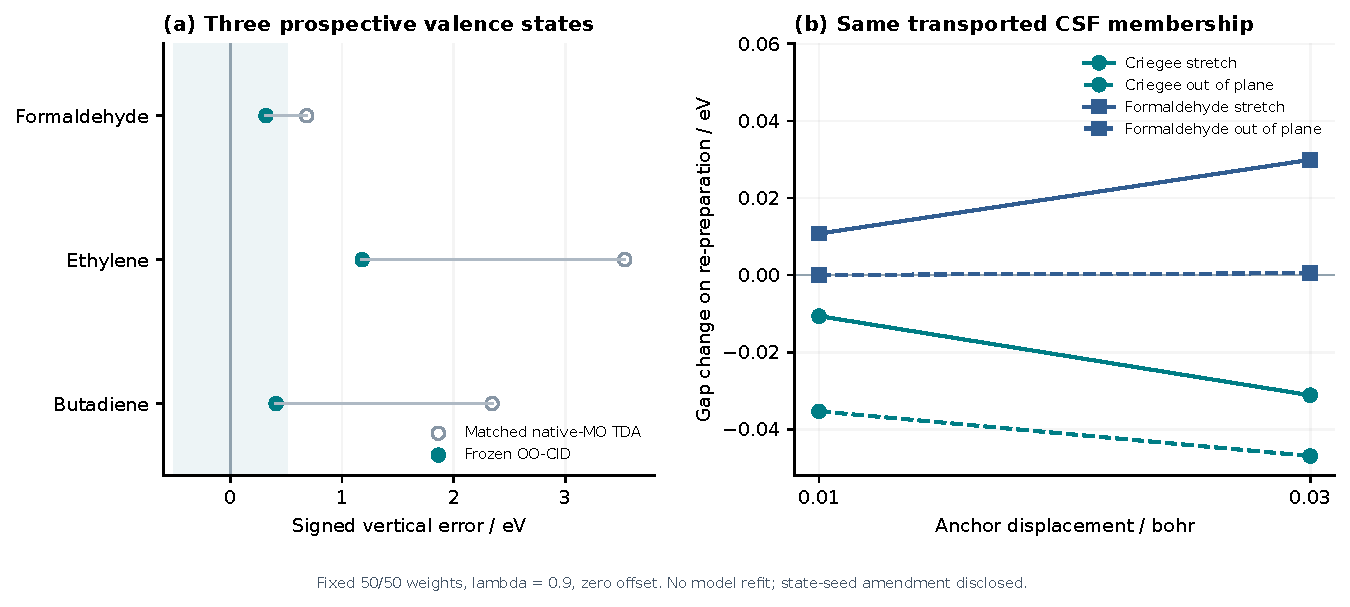
\includegraphics[width=\linewidth]{figures/closing_validation.pdf}
\caption{Final prospective extension and reference-geometry sensitivity.
(a) OO-CID and matched native-orbital TDA signed errors for every new state;
the shaded region is $\pm0.5$ eV. (b) Re-prepared versus original-anchor
excitation gaps evaluated at identical displaced geometries, with the
original CSF membership transported by occupied/virtual orbital overlap.
The model parameters are unchanged. The small extension is separate from
the exposed twenty-state development set.}\label{fig:closingvalidation}
\end{figure}

Anchor tests displace one carbon by 0.01 and 0.03 bohr in an in-plane
stretch or an out-of-plane direction, for the Criegee intermediate and
formaldehyde. Each comparison uses the same physical final geometry,
retains all originally prepared target states and reuses the completed
reference checkpoints. With the original CSF membership transported by
orbital overlap, the largest gap change is 0.047 eV for the Criegee
$\pi\pi^*$ state and 0.030 eV for formaldehyde. These are local controls,
not a bound on arbitrary anchor displacement. Re-selecting the configuration
space at each new anchor is a different operation: loss of the Criegee
reflection certificate reduces its space from 178 to 13 CSFs and changes
the $\pi\pi^*$ gap by 0.263--0.273 eV. A trajectory must retain its frozen
chart; symmetry-dependent space selection must not be silently reapplied
at every displaced geometry. The implemented analytic surface already
retains this membership during nuclear motion.

\subsection{Predecessor structures, frequencies and exact acceleration}
The frozen screened-even predecessor was optimized on the lowest singlet surfaces of
formaldehyde and acetaldehyde using analytic gradients. Full analytic
Hessians then assess the vibrational curvatures. Coupled-cluster internal
coordinates provide a physical structural comparison,\cite{geometries2017}
and selected experimental vibrational fundamentals provide a separately
identified spectroscopic comparison.\cite{formaldehydespectrum1969,acetaldehydespectrum1981}
The model frequencies are unscaled harmonic curvatures, whereas the
experimental numbers are anharmonic level spacings. Modes are assigned
through projections on mass-weighted chemical-coordinate displacement
patterns, rather than matched by frequency order. Inversion splittings and
methyl-torsion level spacings are not used as harmonic curvature references.
Complete coordinates, modes and individual differences are given in the
Supporting Information. These comparisons assess that predecessor energy;
they are not substituted for equilibrium data of the subsequently corrected reference.

A further exact response optimization vectorizes the overlap-residual
completion and avoids scalar derivative-jet allocation for frozen
auxiliary matrix values. A cold two-thread Criegee public-API Hessian takes
397 s, compared with the archived 418 s; energies, gradients and both full
Hessians are bitwise identical between versions. Peak resident memory is
1.19 GB, compared with 1.06 GB. This single-run 4.9\% time reduction is
modest, with other work active on the host, and is not evidence of a
size-scaling improvement or a speed advantage over TDA. The ten algebra,
spin and legacy-contract regressions also pass. No numerical derivative,
Hamiltonian change or fitted correction enters the acceleration.

\subsection{Resolving the ethylene extension with a common screened reference}
The prospective ethylene discrepancy motivates a second, separately
identified development candidate. The F reference represents the full DFT
Fock operator in a confined valence image, whereas its qualified Q levels
come from the larger DFT calculation. To assess this imbalance, let $P$
be the isometric native-valence image and $Q$ its orthogonal complement
in the complete DFT orbital space. For an already qualified orbital match,
we evaluate the diagonal complement self-energy
\begin{equation}
 \Sigma_i(E_i)=F_{iQ}(E_i-F_{QQ})^{-1}F_{Qi}
\end{equation}
at its matched DFT orbital energy and add it to the F level before the
unchanged 50/50 average. Unqualified matches retain their original reference.
This is a diagonal downfolding approximation, not an exact many-electron
elimination of the DFT environment. No excitation reference enters this
one-body preparation. It lowers the ethylene result from 9.079 to 8.206 eV,
consistent with a substantial confinement contribution to the initial error.

The environment screening is rebuilt using Coulomb vertices between native
occupied orbitals and an explicit orthogonal DFT bath, avoiding the use of
missing active-orbital spectral weight as an independent screening channel.
Subspace disentanglement is a recognized issue in constrained
screening.\cite{miyake2009} We allow one global semiempirical efficiency
$\eta$ for this additional bath polarization:
\begin{equation}
 W=L_P^\mathrm{T}
 \left[I+B_NB_N^\mathrm{T}+\eta B_BB_B^\mathrm{T}\right]^{-1}L_P .
\end{equation}
Here $B_N$ contains the retained native environment transitions, $B_B$
the occupied--bath transitions, and $L_P$ the native Coulomb vertices.
The one-body interaction is normal ordered to the corrected native ground
Fock. The retained configuration space is unchanged. Static screening is
an approximation whose quantitative limitations also arise in molecular
RPA downfolding.\cite{verzijl2026}

We calibrate $\eta=0.60$ by balancing the opposite errors of furan V010
and furofuran C002, and freeze it before evaluating the complete ledger.
This is \emph{one fitted interaction parameter}; it is neither an energy
offset nor a parameter-free correction. It applies to every molecule and
state. The F/Q weights stay 50/50, exchange-response $\lambda$ stays 0.9,
and orbital gaps are not multiplied by either parameter. All 23 numerical
labels have been exposed during development, including the three-state
extension, so this assessment is not a blind validation.

\begin{figure}[!htbp]
\centering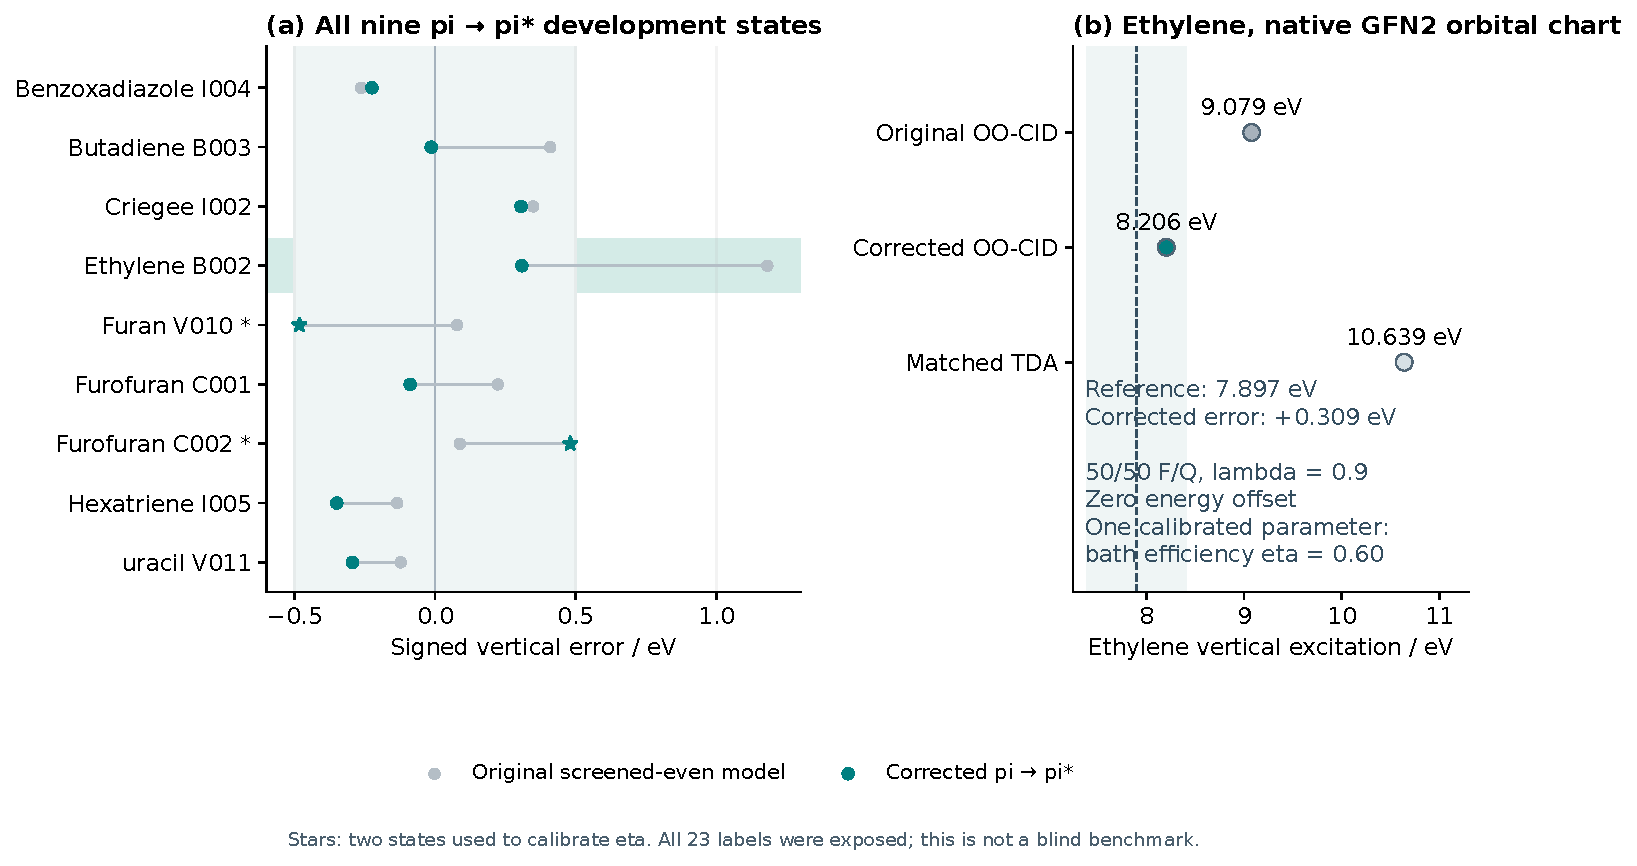
\includegraphics[width=\linewidth]{figures/ethylene_repair.pdf}
\caption{Common-reference repair on the complete exposed development set.
(a) Original and corrected signed errors for all nine $\pi\pi^*$ states; stars identify
the two states used to calibrate bath efficiency $\eta$. (b) Ethylene's
initial and corrected OO-CID energies, with a freshly evaluated TDA control
using the corrected native GFN2 ground orbitals and reference response.
The reference is 7.897 eV. The shaded intervals are $\pm0.5$ eV.}
\label{fig:ethylenerepair}
\end{figure}

All nine $\pi\pi^*$ states now lie within 0.5 eV, with MAE 0.283 eV and
maximum error 0.482 eV. The fourteen $n\pi^*$ states give 0.175 eV MAE
and 0.381 eV maximum error. All 23 states give 0.217 eV MAE. The 21 states
not used to choose $\eta$ give 0.192 eV MAE; their earlier exposure still
precludes a blind-validation claim. The matched corrected-reference TDA
MAEs are 1.726 eV for $\pi\pi^*$, 0.174 eV for $n\pi^*$ and 0.781 eV
overall. Thus the measured accuracy benefit is concentrated in $\pi\pi^*$;
the two $n\pi^*$ mean errors are essentially equal. This response control
is not a separately optimized published TDA parameterization.

Ethylene has error $+0.309$ eV. Its full analytic Hessian takes 10.15 s on
the verified two-thread Mac Studio run; two independent scalar-energy
Richardson checks give maximum errors $1.73\times10^{-11}$ Ha/bohr for
the gradient and $6.56\times10^{-8}$ Ha/bohr$^2$ for directional curvature.
The coherent singlet has $\langle S^2\rangle=0$, and its accepted restart
agrees within $8.9\times10^{-16}$ Ha. No DFT import, TDA solve or new SCC
driver is used during prepared evaluation. These derivatives belong to the
corrected frozen anchored surface. The earlier minimum and frequency
comparisons in the preceding subsection belong to its screened-even
predecessor and are not reassigned to this calibrated extension. Independent
prospective molecules and corrected-model equilibrium structures remain
necessary before a general transferability claim.

\subsection{Fragmented orbital matches and three further valence tests}
The fixed $\eta=0.60$ candidate is next applied to cyclopropene,
cyclopentadiene, and pyrrole. All three predictions are archived before
extracting their numerical QUEST references. Their errors are initially
$+0.054$, $-0.013$, and $+2.369$ eV. Historical exposure of some of these
molecules prevents a strictly blind claim. Pyrrole's discrepancy exposes
a reference-construction limitation: its native virtual orbitals have
substantial weight distributed over several full-DFT virtual orbitals,
so no individual match meets the existing 0.7 amplitude criterion.
The original fallback therefore omits both the qualified Q level and the
complement relaxation for these orbitals.

We amend this rule for \emph{every} unresolved occupied or virtual orbital,
without a molecule or state-family branch. Within the same occupation
sector, full-DFT poles are ordered by native spectral weight $w_{ki}$.
The smallest block $\mathcal B_i$ satisfying
$\sum_{k\in\mathcal B_i}w_{ki}\geq0.7^2$ supplies the normalized centroid
\begin{equation}
 \mu_i=\frac{\sum_{k\in\mathcal B_i}w_{ki}\epsilon_k}
 {\sum_{k\in\mathcal B_i}w_{ki}} .
\end{equation}
This centroid supplies the Q level with the original occupied-centroid
alignment. Its difference from the Rayleigh energy of the original
native image supplies the unresolved F relaxation. Individually qualified
poles retain their preceding treatment. We then rebuild the explicit
bath screening on the corrected native orbitals. The 50/50 average,
$\lambda=0.9$, $\eta=0.60$, configuration rule and zero energy offset remain
fixed. This is a diagonal spectral-centroid approximation, not an exact
elimination of a broad or frequency-dependent environment. The reference
preparer reads no excitation labels, but the amendment was developed after
pyrrole scoring: the resulting ledger is an exposed development assessment.

Pyrrole then gives 6.302 eV against 6.247 eV. Applying the identical rule
to all 26 states in 24 molecules gives MAE 0.198 eV and maximum error
0.446 eV. The twelve $\pi\pi^*$ states give 0.216 eV MAE; the fourteen
$n\pi^*$ states give 0.183 eV. All individual errors are below 0.5 eV.
Matched TDA on the corrected native GFN2 orbitals gives 0.789 eV MAE
overall, 1.514 eV for $\pi\pi^*$ and 0.168 eV for $n\pi^*$: the OO gain
is concentrated in the $\pi\pi^*$ family, while TDA has the smaller mean
$n\pi^*$ error. Neither comparison is a calibrated sTDA-xTB benchmark.
Every prepared state passes fresh-process spin and restart checks with no
DFT import, new SCC call or TDA solve. Ethylene's updated full analytic
Hessian takes 10.68 s; scalar-energy Richardson checks give errors below
$9.92\times10^{-12}$ Ha/bohr and $2.46\times10^{-8}$ Ha/bohr$^2$.
These remain derivatives of a frozen anchored model.

\begin{figure}[!htbp]\centering
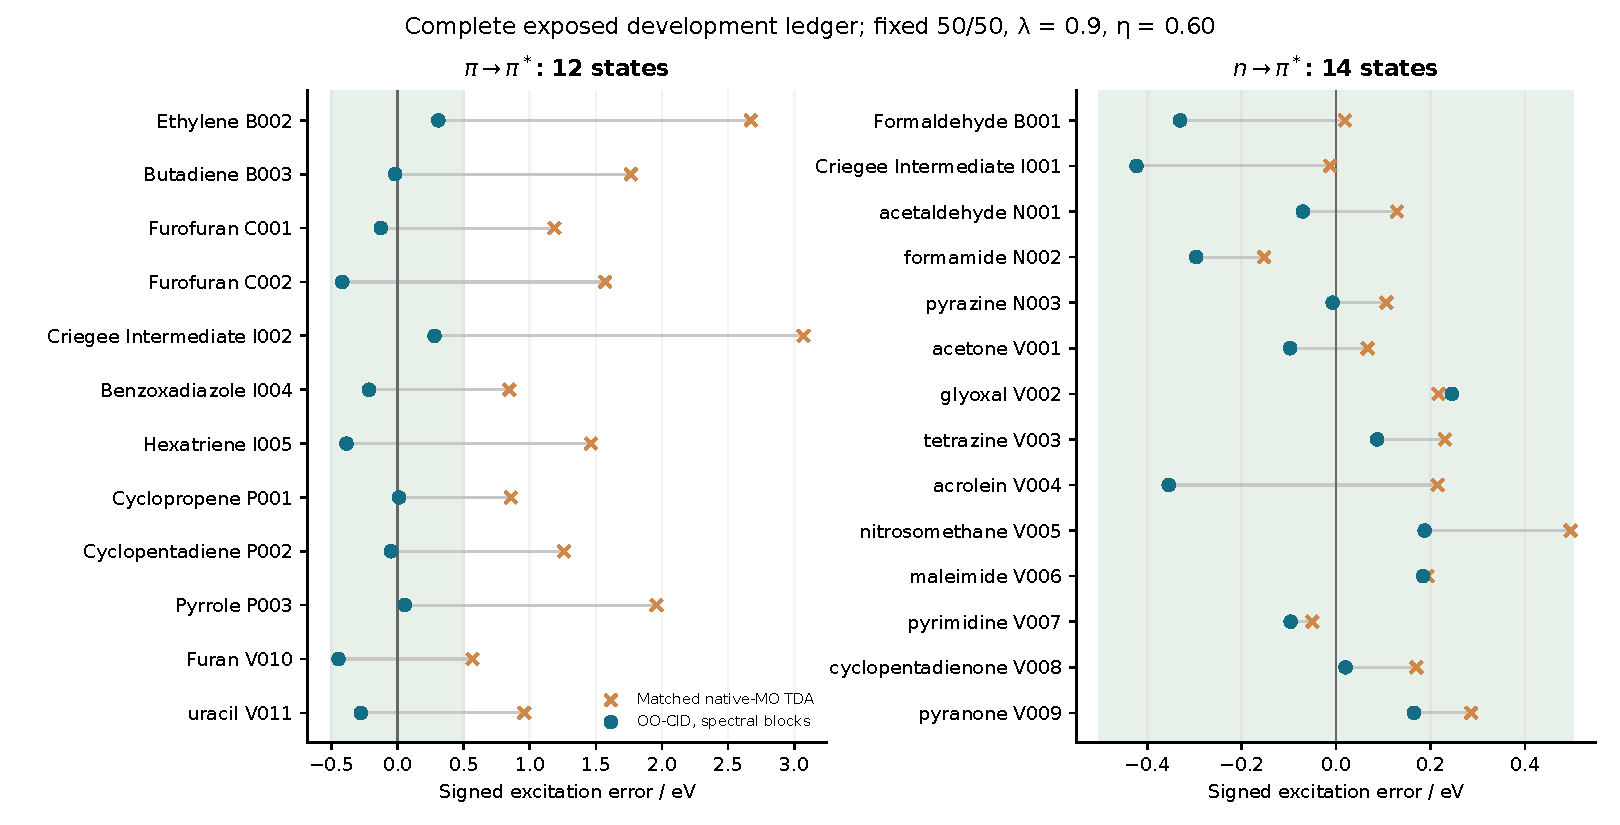
\includegraphics[width=\linewidth]{figures/spectral_block_validation.pdf}
\caption{All 26 exposed development states after the generic spectral-block
reference amendment. Points compare OO-CID with freshly calculated TDA on
the same corrected native orbitals. The shaded interval is $\pm0.5$ eV.
The two panels use different horizontal scales. Neither the bath efficiency
nor the F/Q weights are retuned for the three added molecules.}
\label{fig:spectralblocks}
\end{figure}

\subsection{Larger pigment structures: preparation scope}
We select all-trans $\beta$-carotene and chlorophyllide a as larger
chromophore tests. Chlorophyllide a retains Mg and the conjugated
substituents while removing the phytyl chain. Figure~\ref{fig:pigmentstructures}
shows the actual source structures, rather than schematic molecular art.
Native ground checkpoints contain 216 and 219 orbitals, respectively.
The chlorophyllide reconstruction explicitly includes Mg d functions.
Raw Gaussian-overlap discrepancies and subsequent numerical metric
reconciliation are archived separately; agreement after reconciliation is
$2.5\times10^{-13}$ or better. The one-time PBE0/CAM-B3LYP reference
preparation uses checkpointed RI-JK calculations on the verified Mac Studio.
No pigment excitation energy, excited minimum or Hessian is claimed here,
and these molecules are excluded from the 26-state accuracy pool.
Nonplanar configuration selection, the distinction between dark and bright
carotenoid states, and mixing of chlorophyll Q-band targets require explicit
qualification before extending the model's demonstrated scope.

\begin{figure}[p]\centering
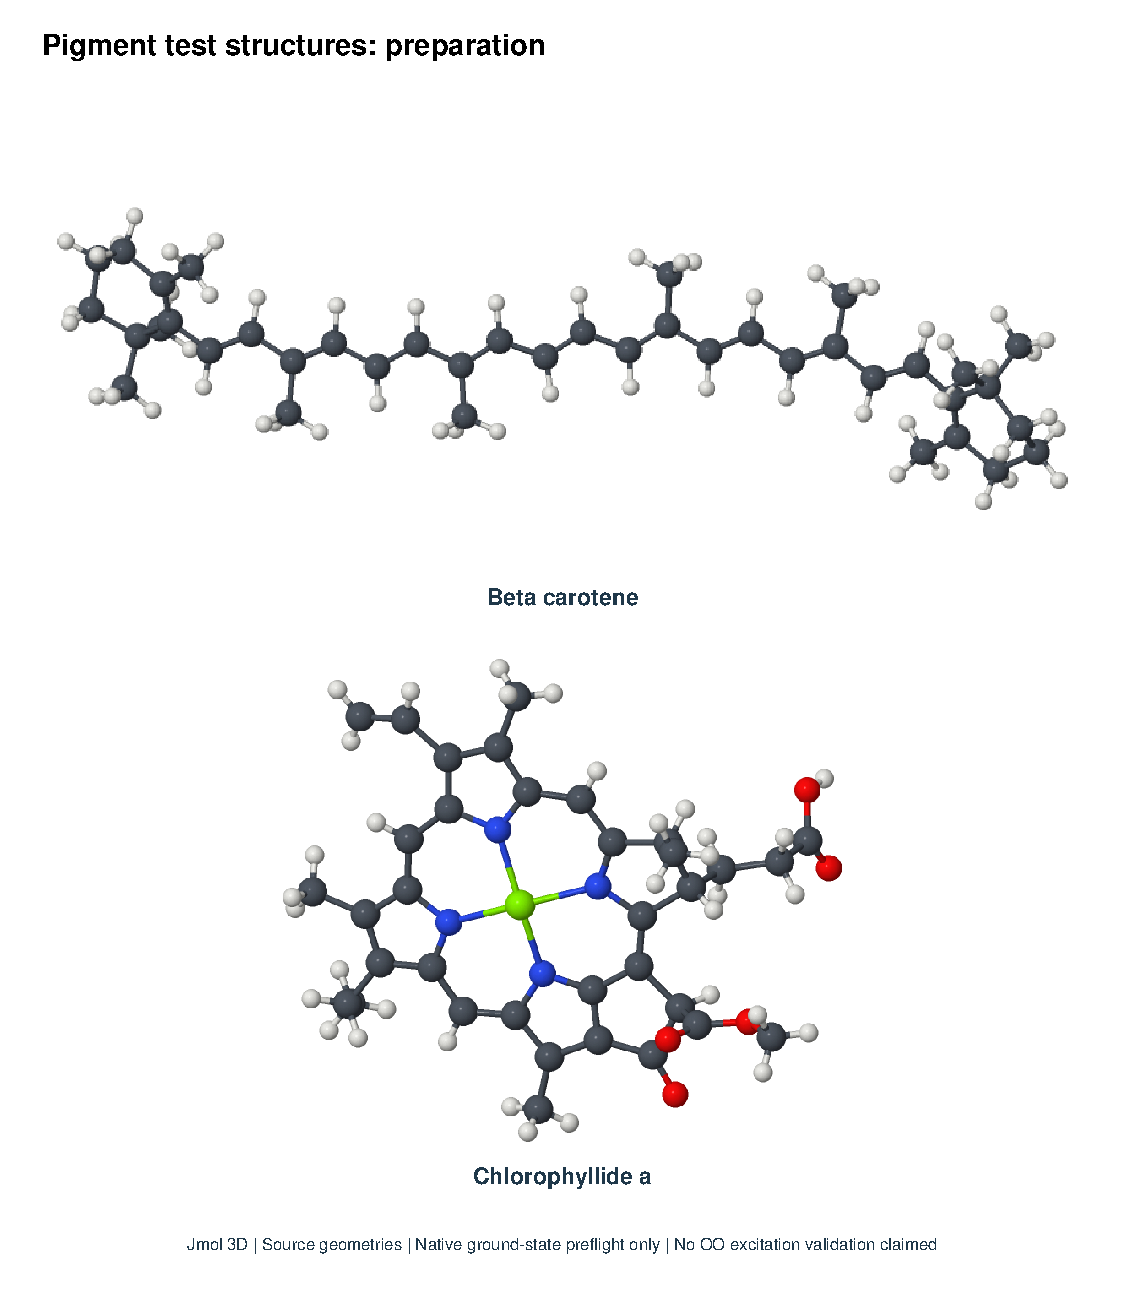
\includegraphics[width=.92\linewidth,height=.80\textheight,keepaspectratio]{figures/pigment_test_structures_jmol.pdf}
\caption{Jmol renderings of the larger starting structures: all-trans
$\beta$-carotene (96 atoms; PubChem CID 5280489) and chlorophyllide a
(79 atoms; RCSB ligand A1JWG). These primary-source geometries are used
for preparation and are not optimized excited-state structures or
validated additions to the accuracy ledger.}
\label{fig:pigmentstructures}
\end{figure}

\subsection{Static matching of the extended configuration interaction}
Adding explicit configuration interaction to density-functional diagonal
energies requires deciding which correlation is already represented.
DFT/MRCI addresses this
issue through an effective Hamiltonian with empirical damping.\cite{marian2019mrci}
We examine zero-frequency self-energy subtraction, following its use in
extended response theories.\cite{tselyaev2013,gambacurta2015}
The borrowed principle is static matching. Its molecular OO-CID application
is a development proposal, rather than an exact density-functional result.

After removing the native ground CSF, define
$\widetilde H=P_g^\dagger(H-E_gS)P_g$ and
$\widetilde S=P_g^\dagger SP_g$. The fixed primary space contains the
optimized singlets and their paired partners; the complementary space
contains all canonical auxiliary configurations. Metric orthogonalization
of the latter gives
\begin{align}
 X&=\widetilde S_{PP}^{-1}\widetilde S_{PQ},\qquad
 A=\widetilde H_{PP},\qquad V=\widetilde H_{PQ}-AX,\\
 D&=\widetilde H_{QQ}-\widetilde H_{QP}X
       -X^\dagger\widetilde H_{PQ}+X^\dagger AX.
\end{align}
Adding $VD^{-1}V^\dagger$ to the primary block in these coordinates yields
\begin{equation}
 H_{\mathrm{eff}}^{\mathrm{sub}}(\omega)
 =A+VD^{-1}V^\dagger+V(\omega S_Q-D)^{-1}V^\dagger,
 \qquad H_{\mathrm{eff}}^{\mathrm{sub}}(0)=A ,
\end{equation}
where $S_Q=\widetilde S_{QQ}-\widetilde S_{QP}X$.
The complete interacting $D$ is used, rather than its diagonal. Its
positivity is checked before inversion. No damping coefficient, constant
excitation shift or orbital-reference adjustment is fitted. The 50/50
weights, $\lambda=0.9$ and previously calibrated $\eta=0.60$ are unchanged.

On the same 26 exposed states, the MAE changes from 0.198 to 0.183 eV.
The $\pi\pi^*$ and $n\pi^*$ MAEs become 0.209 and 0.160 eV. The maximum
individual error increases from 0.446 to 0.478 eV; all errors remain
below 0.5 eV. Table~\ref{tab:staticmatching} and
Figure~\ref{fig:staticmatching} show both the mean improvement and the
cases that become less accurate. All 24 models reproduce these energies
through the public API, with coherent-singlet spin and accepted-restart
checks. These exposed labels do not provide independent transferability
validation.
\begin{table}[!htbp]\centering\small
\caption{Static-matching development candidate on the same corrected native orbitals, geometries and 26 exposed reference labels. No parameter is refitted. All errors are in eV.}
\label{tab:staticmatching}
\begin{tabular}{lrrrrr}\toprule
Family & States & TDA MAE & Before MAE & Matched MAE & Matched max.\\\midrule
All & 26 & 0.789 & 0.198 & 0.183 & 0.478\\
$\pi\pi^*$ & 12 & 1.514 & 0.216 & 0.209 & 0.478\\
$n\pi^*$ & 14 & 0.168 & 0.183 & 0.160 & 0.411\\
\bottomrule\end{tabular}
\end{table}

\begin{figure}[!htbp]\centering
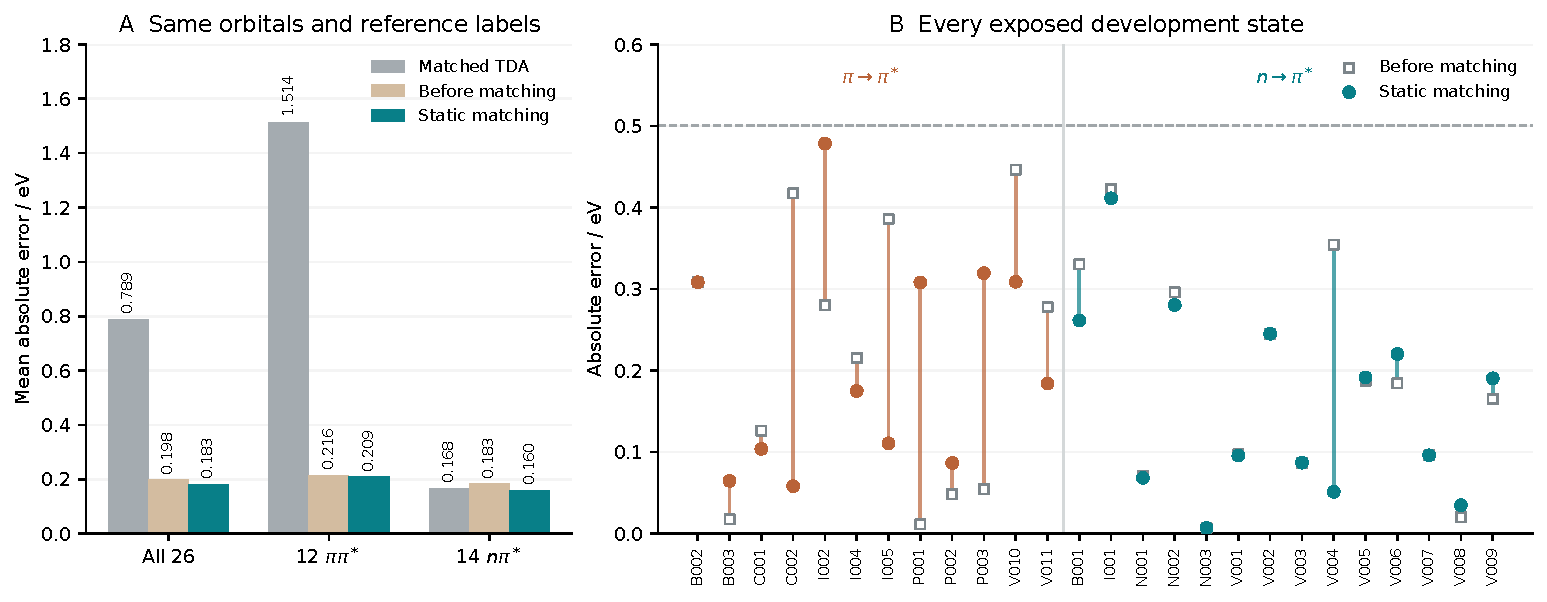
\includegraphics[width=\linewidth]{figures/static_subtraction_accuracy.pdf}
\caption{Static matching on the unchanged exposed development set.
(A) Family-resolved MAEs compared with the unsubtracted candidate and
matched TDA on the same corrected native GFN2 orbitals. (B) Every individual
absolute error before and after matching. The dashed line marks 0.5 eV.
No parameter is refitted and no molecule or state-family branch is added.
This is a development comparison rather than blind validation.}
\label{fig:staticmatching}
\end{figure}

The counterterm participates in the complete analytic nuclear response.
Both derivatives of $D^{-1}$, the metric orthogonalization, the moving
ground projector and $E_g$ are differentiated. Freezing this counterterm
after its vertical evaluation would define a different surface.
The checksummed manifest field
\texttt{static\_self\_energy\_subtraction} selects this candidate through
the existing MOUSE/LINK interface. Older manifests retain their original
Hamiltonian and restart identity. Ethylene's full analytic Hessian takes
9.82 s in a two-thread run. Independent reconverged scalar-energy checks
give maximum directional gradient and curvature errors of
$1.9\times10^{-11}$ Ha/bohr and $3.1\times10^{-8}$ Ha/bohr$^2$.
Furan's complete 27-coordinate Hessian takes 1386.40 s in the serial
column implementation and 297.18 s with eight worker processes (4.67-fold
wall-time reduction). The complete energy, gradient and Hessian arrays
agree exactly between these runs. The serial surface passes independent
scalar-energy checks with maximum gradient and curvature errors of
$1.2\times10^{-10}$ Ha/bohr and $6.6\times10^{-8}$ Ha/bohr$^2$.
Workers reuse the converged orbital states and differentiate the analytic
response columns; no electronic reoptimization is repeated per column.
These timings exclude reference preparation and are not speedup claims
against TDA. Finite differences enter validation only.

The pigment extension tests a different aspect. At the matched
13-orbital frontier, $\beta$-carotene retains a weak lowest state at
2.244 eV ($f=1.58\times10^{-4}$), followed by a dominant absorbing
root at 3.031 eV ($f=5.00$). The bright state is root 4; root 3 at
2.875 eV is weak. This assignment uses recomputed transition moments,
whose unsubtracted replay exactly reproduces the stored convention.
The chlorophyllide lowest gaps at $N=W=16$ become 2.019 and 2.226 eV,
instead of 1.246 and 1.425 eV before matching. These changes are not
a constant shift. The first two roots satisfy the two-increment 0.02 eV
test over $N=14,15,16$ in both matched and fixed-screening sequences.
Higher roots require further frontier and target-coverage checks; a fully
converged static-matched chlorophyllide spectrum is not yet claimed.
Neither pigment enters the 26-state accuracy statistics, and the pigment
adapter does not supply qualified nuclear derivatives.


The next scientific assessment should test the calibrated correction on
independent molecules, additional CT and Rydberg states, corrected-model
equilibrium structures, and larger nuclear displacements.
The prospective and structural controls reported here limit the scope of
the finite development result; they do not establish universal transferability.

\section{Conclusions}
MOUSE provides a semiempirical orbital-optimized route with explicit spin
polarization, spin-pure singlet CSFs, and analytic nuclear gradients and
Hessians. Ground-program Fock, energy and derivative primitives are reused
through constrained electronic saddle optimization and implicit response.
The current candidate combines a spectral-block orbital reference,
selected screened double excitations and zero-frequency self-energy
matching with fixed F/Q weights of 50/50,
exchange-response scale 0.9 and one calibrated bath efficiency,
$\eta=0.60$. No excitation-energy offset is fitted. Across 26 states in 24
molecules it gives 0.183 eV MAE and 0.478 eV
maximum error. The twelve $\pi\pi^*$ states give 0.209 eV MAE, compared
with 1.514 eV for TDA on the same corrected native GFN2 orbitals. For the
fourteen $n\pi^*$ states, the corresponding values are 0.160 and
0.168 eV, respectively. The same state-specific surface describes the
excitation energy, orbital relaxation and nuclear response.

The prepared surface retains coherent APOC state following and accepted-only
LINK restarts without a runtime TDA solve, new SCC call or DFT-backend
import. Complete implicit response differentiates the anchored energy,
the moving ground projector and the state-interaction eigensystem.
Independent energy checks support the analytic derivatives; the ethylene full
Hessian takes 9.82 s in one two-thread run. The resulting gradients and
curvatures provide the quantities needed for excited-state relaxation and
vibrational analysis.

Matrix-free orbital stationarity and exact frozen-quadrature XC correction
extend the numerical implementation to larger native valence spaces. The
carotene configuration expansion keeps a weak first singlet below the
absorbing manifold without parameter adjustment. The matched 13+13
frontier uses 14,535 CSFs. Static matching retains a weak first gap at
2.244 eV and a dominant fourth-root absorption at 3.031 eV. The two lowest
chlorophyllide gaps are 2.019 and 2.226 eV and satisfy the two-increment
0.02 eV convergence check.
Collective target-space tracking follows absorbing subspaces through
mixing. These pigment calculations extend the method to strongly conjugated
visible chromophores and define applications to excited-state structures and
vibronic spectra.
The full-DFT DeltaSCF/ROKS implementation developed in parallel, including
analytic nuclear response, is intentionally outside the scope of this
semiempirical manuscript and will be reported as a separate companion work.

\section*{Data and software availability}
MOUSE source is hosted at \url{https://github.com/yogibubu/MOUSE}.
The final symmetry-augmentation choice is frozen in \texttt{2d59ab8}; the
portable surface and analytic response are implemented in \texttt{81897cf},
with exact contraction/metric acceleration in \texttt{e572d50}.
The closing protocol is frozen in \texttt{94d2312}, with exact dense
response acceleration in \texttt{67c835f}. Its new cases, reference-geometry
controls and molecular minima are archived in
\path{qualification/closing_validation_20261101}.
The calibrated bath protocol is frozen in \texttt{8f95105}; its complete
23-state ledger, matched corrected-reference TDA and ethylene derivative
certificate are in \path{qualification/closing_validation_20261101}.
Original twenty-state qualification and its complete logs are committed in \texttt{358ae21}
and \texttt{7c5c7f9}. The qualification directory
\path{qualification/pi_pi_transfer_repair_20261101}
contains the complete twenty-state predictions, model/exposure protocol,
remote runtime and spin checks, analytic-column checkpoints, independent
energy validations and executed-source hashes. The manuscript package
contains the machine-readable results, scientific figure sources, archived
Jmol renders and coordinate provenance. Earlier generations and their
qualification archives are identified separately in the Supporting Information
and preserved development manuscript. The large-system runtime and exact accelerations are archived in
\texttt{d05afa6} and \texttt{e3c005a}, with fragmented-target tracking
in \texttt{bb3435f}. The compiled integer-mask kernel and iterative CI
solver are in \texttt{9248a39}; consistent observable phases and reuse of
native functional values are in \texttt{8d44bb3}. The coherent-window
convergence audit is in \texttt{cc1a5c2}, with complete evidence in
\texttt{0fb963f}. Large pigment checkpoints remain on the verified
compute host with checksummed receipts and compact low-state exports.
A permanent public dataset identifier
has not yet been assigned.

\section*{Author contributions}
V.B. conceived the method, developed the implementation and validation
protocol, analyzed the results, and wrote the manuscript and Supporting
Information.

\section*{Conflict of interest}
The author declares no conflict of interest.

\section*{Data availability}
All source code, input geometries, machine-readable data, figures and
qualification records needed to reproduce the reported calculations are
included in the MOUSE repository and identified by the commit and archive
paths given above. Large pigment checkpoints are retained on the verified
compute host with checksummed receipts; a public dataset DOI will be added
before publication.

\section*{Graphical abstract}
\begin{center}
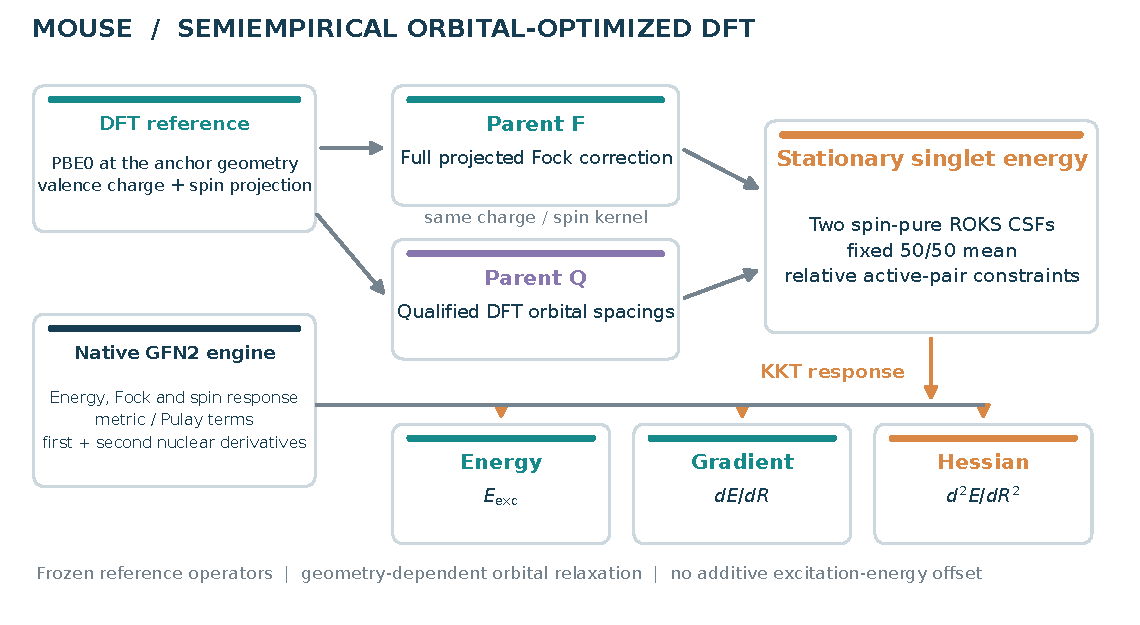
\includegraphics[width=0.82\linewidth]{figures/method_workflow.pdf}
\end{center}
\noindent\emph{TOC text:} A prepared DFT-informed semiempirical surface
combines spin-pure orbital optimization, coherent state interaction and
analytic nuclear response for repeated excited-state calculations.

\setlength{\bibsep}{2pt}
\bibliographystyle{unsrtnat}
\bibliography{references}
\end{document}
